\section{Four-Task Study Design}\label{sec:design}

The four tasks are not identical in dataset, label space, objective, or metric -- Task 1 has
no graph at all, Task 2 is single-label classification on GTZAN, Task 3 is multi-label
classification on MusicCaps, and Task 4 is a ranking objective with no genre or tag class
labels, using audio-caption pair identity as supervision. What they do
share is the node-feature definition (32-dimensional chroma plus MFCC), the same
similarity-based graph construction rule, and closely matched encoder architectures where a
graph is involved; Task 4 was also built in a separate implementation with a different
segment length and dataset split (Section~\ref{sec:data} discloses this precisely). This
shared representation is what makes a cross-task comparison informative at all: each task's
own graph-vs-edge-free result is its own self-contained comparison, with its own explicitly
disclosed matching exceptions (Section~\ref{sec:protocol}) rather than a uniform fairness
guarantee across tasks, and it
is the \emph{consistency of the overall conclusion} those results support -- not an
identical numeric comparison in every task, and not an assumption that every task used
byte-identical inputs -- that the cross-task analysis in Section~\ref{sec:cross-task} relies
on.

\textbf{Task 1 -- Text Tag Prediction.} A text-only reference point. A BERT-family encoder
predicts tags from a caption alone, with no audio and no graph at all. This establishes how
much of the target signal language already carries by itself -- a qualitative anchor for the
rest of the paper's "does the graph add anything" question, not a numerical baseline every
later task's own metric is scored against, since Task 2 uses a different dataset and label
space and Task 4 uses a different metric entirely.

\textbf{Task 2 -- Graph-Based Audio Classification.} A graph neural network predicts genre
from an audio-only segment graph, compared against (a) a non-graph CNN baseline operating
directly on the log-mel spectrogram, and (b) a width/depth-matched, lower-parameter, edge-free
encoder using the exact same node features as the graph model, with every edge removed.
Comparison (b) tests whether the graph encoder, as a whole, adds anything over a
structure-free alternative; because it changes the aggregation operator along with the
edges, it does not isolate topology alone -- Section~\ref{sec:results-t2} also reports a
same-architecture, edges-only intervention from a companion audit for that narrower
question.

\textbf{Task 3 -- Multimodal Context Prediction.} A graph encoder of the same architecture as
Task 2's is fused with a separately initialized instance of the same pretrained text-encoder
architecture used in Task 1 (not Task 1's own trained weights), compared across four fusion
strategies (text-only, graph-only,
concatenation, cross-attention) plus two diagnostics: zeroing the graph branch inside a
trained fusion model, and cross-tabulating which examples the text-only and graph-only
models get right or wrong. This tests whether the graph is complementary to text, not just
whether it is useful on its own.

\textbf{Task 4 -- Audio-Text Retrieval.} A contrastive dual encoder learns to match a
caption to its audio clip, with no genre or tag class labels, using only audio-caption
pairing as supervision -- a different objective from classification,
scored by ranking (Recall@K) rather than accuracy. The same graph-vs-edge-free comparison
from Task 2 is repeated here, to test whether any graph advantage (or its absence) generalizes
beyond classification to a fundamentally different task type.

Figure~\ref{fig:progression} summarizes the ladder: each task adds one element -- audio,
fusion, then a different objective -- while keeping the node-feature definition and graph
construction rule fixed (Section~\ref{sec:data} discloses where the underlying
implementation still differs between tasks).

\begin{figure}[t]
\centering
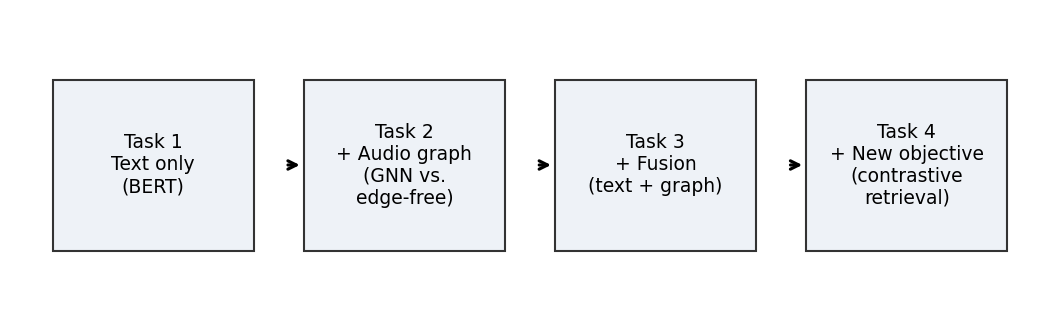
\includegraphics[width=0.95\columnwidth]{figures/fig1_progression.png}
\caption{The four-task progression. Each task keeps the same node features and graph
construction rule, and adds one new element: audio (Task 2), fusion with text (Task 3), or a
different objective (Task 4).}
\label{fig:progression}
\end{figure}
